\section{SR reachability}

In this section we focus on trying to understand how costly, in terms of segments, it is to connect two
nodes with a deterministic sr-path. These results are very useful in order to provide lower bounds on the 
minimum cost of any segmentation of a path between two given nodes.
% 
% As we have seen already in numerous examples, sr-paths can correspond to a lot a paths in the original netwoks.
% For this reason, it is not always possible to know exactly which links are traversed. This can be problematic in
% some applications. For instance, imagine that you use a sr-path $\sr{p}$ to communicate between two nodes. If $\sr{p}$
% correspond to several paths in the original network $G$, one cannot even tell with certainty what is the latency 
% of this path. All we can do is give a bound and say that it is at most the slowest of all paths represented by $\sr{p}$.
% In our network monitoring chapter we will see another example where this uncertainty is problematic.
% 
% This motivates the definition of determinism for a sr-path. 
% 
% \begin{definition}
% A sr-path $\sr{p} = \langle x_1, \ldots, x_l \rangle$ is said to be deterministic if for each $i \in \{2, \ldots, l\}$
% there exists a unique IGP shortest path between $x^2_{i - 1}$ and $x^1_i$, that is, $\sp(x^2_{i - 1}, x^1_i)$ is a path
% in $G$.
% \end{definition}




%\begin{definition}
%Let $G$ be a network, $s \in V(G)$ and $k \geq 0$ an integer. We define the deterministic node reachability of $v$ with cost
%at most $k$ as
%$$
%\nreach(k, s) = \left\{ v \in V(\sr{p}) \mid \textrm{$\sr{p}$ is a deterministic sr-path starting at $s$ with $\cost(\sr{p}) \leq k$} \right\}
%$$
%\end{definition}

%---------------------------------------------------------------------------------------------------

% \begin{definition}
% Let $G$ be a network and $s \in V(G)$. For any integer $k \geq 1$ we define
% \begin{align*}
% \nreach^n(k, s) = & \ \textrm{set of nodes $v \in V(G)$ such that there exists a deterministic} \\ 
%                 & \ \textrm{sr-path $\sr{p} = \langle x_1, \ldots, x_l, v \rangle$ of segment cost at most $k$},
% \end{align*}
% \begin{align*}
% \nreach^e(k, s) = & \ \textrm{set of nodes $v \in V(G)$ such that there exists a deterministic} \\ 
%                   & \ \textrm{sr-path $\sr{p} = \langle x_1, \ldots, x_l, (u, v) \rangle$ of segment cost at most $k$}
% \end{align*}
% and
% $$
% \nreach(k, s) = \nreach^n(k, s) \cup \nreach^e(k, s)
% $$
% \end{definition}

Since segment routing is a new technology, network topologies were not designed with SR in mind.
Therefore it could very well be the case that current topologies require very long lists of segments
to represent specific paths. For this reason we would like to have tools to analyse
a given topology to see how suitable it is for SR. Consider the topology shown in Figure \ref{fig:reach-ex1}.
If we follow shortest paths starting from router \node{e} (in green) and restrict ourselves to only visiting nodes
whose shortest path from \node{e} is unique, then we will only be able to reach nodes \node{a}, \node{b},
\node{d}, \node{f}, \node{h} and \node{i} (in gray). Thus we can already say about this topology that
it needs at least sr-paths of cost $3$ to reach any given node with a deterministic sr-path from \node{e}.
In other words, there exists a simple path starting at \node{e} that needs at least $3$ segments to be represented with
segment routing.

\begin{figure}[H]
\begin{center}
\begin{tikzpicture}
\def\x{0}
\def\y{0}
\node[scale=0.15] (a) at (0.5 + \x,  0.5 + \y) {\router{a}{marked}};
\node[scale=0.15] (b) at (0.5 + \x, -1.0 + \y) {\router{b}{marked}};
\node[scale=0.15] (c) at (2.5 + \x,  0.0 + \y) {\router{c}{router}};
\node[scale=0.15] (d) at (4.5 + \x,  0.0 + \y) {\router{d}{marked}};
\node[scale=0.15] (e) at (4.0 + \x, -2.0 + \y) {\router{e}{green}};
\node[scale=0.15] (g) at (6.0 + \x,  0.5 + \y) {\router{g}{router}};
\node[scale=0.15] (i) at (8.0 + \x,  0.0 + \y) {\router{i}{marked}};
\node[scale=0.15] (h) at (7.0 + \x, -1.5 + \y) {\router{h}{marked}};
\node[scale=0.15] (f) at (4.0 + \x, -3.5 + \y) {\router{f}{marked}};
\node[scale=0.15] (j) at (8.0 + \x, -2.5 + \y) {\router{j}{router}};
\draw[line width=2] (f) edge[above, sloped] node[black,font=\bfseries] {\tiny \texttt{}} (j);
\draw[line width=2] (h) edge[above, sloped] node[black,font=\bfseries] {\tiny \texttt{}} (j);
\draw[line width=2] (a) edge[above, sloped] node[black,font=\bfseries] {\tiny \texttt{}} (b);
\draw[line width=2] (b) edge[above, sloped] node[black,font=\bfseries] {\tiny \texttt{}} (c);
\draw[line width=2] (b) edge[above, sloped] node[black,font=\bfseries] {\tiny \texttt{}} (e);
\draw[line width=2] (b) edge[above, sloped] node[black,font=\bfseries] {\tiny \texttt{}} (f);
\draw[line width=2] (e) edge[above, sloped] node[black,font=\bfseries] {\tiny \texttt{}} (f);
\draw[line width=2] (h) edge[above, sloped] node[black,font=\bfseries] {\tiny \texttt{}} (f);
\draw[line width=2] (g) edge[above, sloped] node[black,font=\bfseries] {\tiny \texttt{}} (i);
\draw[line width=2] (i) edge[above, sloped] node[black,font=\bfseries] {\tiny \texttt{}} (h);
\draw[line width=2]  (d) edge[above, sloped] node[black,font=\bfseries] {\tiny \texttt{}} (g);
\draw[line width=2]  (d) edge[above, sloped] node[black,font=\bfseries] {\tiny \texttt{}} (e);
\draw[line width=2]  (e) edge[above, sloped] node[black,font=\bfseries] {\tiny \texttt{}} (h);
\draw[line width=2]  (g) edge[above, sloped] node[black,font=\bfseries] {\tiny \texttt{}} (h);
\draw[line width=2]  (c) edge[above, sloped] node[black,font=\bfseries] {\tiny \texttt{}} (d);
\draw[line width=2]  (a) edge[above, sloped] node[black,font=\bfseries] {\tiny \texttt{}} (b);
\draw[line width=2]  (a) edge[above, sloped] node[black,font=\bfseries] {\tiny \texttt{}} (c);

%%%%
\draw (e) edge[line width=2, darkgreen, above, ->] (d);
\draw (e) edge[line width=2, darkgreen, above, ->] (b);
\draw (e) edge[line width=2, darkgreen, above, ->] (h);
\draw (e) edge[line width=2, darkgreen, above, ->] (f);
\draw (b) edge[line width=2, darkgreen, above, ->] (a);
\draw (h) edge[line width=2, darkgreen, above, ->] (i);

\end{tikzpicture}
\end{center}
\caption{Shortest path reachability of node \node{e}}.
\label{fig:reach-ex1}
\end{figure}


Of course this topology is very small and thus easy to analyse. To analyse larger topologies, we propose to define the $k$ \emph{deterministic reachability}
of a node as the set nodes that can be reached from it with a deterministic sr-path of segment cost at most $k$. We will then propose 
efficient algorithms for computing these values for any given node $v$ and segment cost $k$.

We start with the definition of shortest path deterministic reachability.

\begin{definition}
\label{def:spreach}
Let $G$ be a netwrok and $v \in V(G)$. We define the \emph{shortest path deterministic reachability} of $v$ as
$$
\spreach(v) = \left\{ u \in V(G) \mid \textrm{there is a unique shortest path between $v$ and $u$} \right\}
$$
\end{definition}

For example, on Figure \ref{fig:reach-ex1} we see that $\spreach(\node{e}) = \{ \node{a}, \node{b}, \node{d}, \node{e}, \node{f}, \node{h}, \node{i} \}$.
As we prove in Theorem \ref{thm:nreach}, this definition constitutes the basic building block that allows to compute the general 
deterministic reachability of a node.

\begin{definition}
Let $G$ be a network and $s \in V(G)$. For any integer $k \geq 1$ we define
\begin{align*}
\nreach(k, s) = & \ \textrm{set of nodes $v \in V(G)$ such that there exists a deterministic} \\ 
                & \ \textrm{sr-path $\sr{p}$ from $s$ to $v$ of segment cost at most $k$}
\end{align*}
% and
% \begin{align*}
% \ereach(k, s) = & \ \textrm{set of edges $e \in E(G)$ such that there exists a deterministic} \\ 
%                 & \ \textrm{sr-path of segment cost at most $k$, $\sr{p} = \langle x_1, \ldots, x_l \rangle$, from} \\
%                 & \ \textrm{$s$ to $u_2$ such that either $e = x_l$ or $x_l$ is a node segment and} \\
%                 & \ \textrm{$e$ is the last edge of the unique shortest path between $x^2_{l - 1}$} \\
%                 & \ \textrm{and $x_l$}
% \end{align*}
\end{definition}

The following theorem provides a recurrence relation for $\nreach(k, s)$ in terms of smaller values of
$k$ and other nodes in the network.


\begin{figure}
\begin{center}
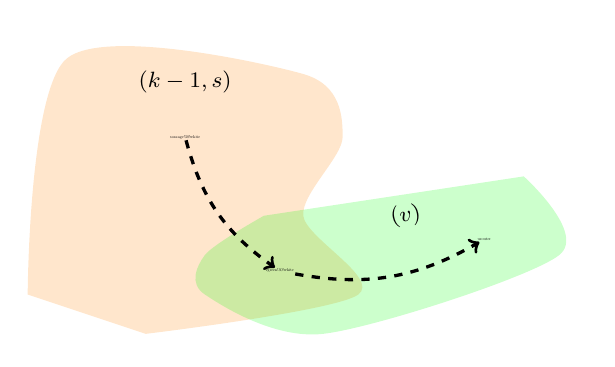
\begin{tikzpicture}
\fill[orange, opacity = 0.2] plot [smooth] coordinates { 
(-1.5, -1) 
(-1, 2) 
(2, 1.8) 
(2.5, 1) 
(2, 0) 
(2.7, -1) 
(0, -1.5)
};

\fill[green, opacity = 0.2, xscale = 1.5] plot [smooth] coordinates { 
(1.5-0.5, 0) 
(1-0.5, -0.5) 
(1-0.5, -1) 
(2-0.5, -1.5)
(4-0.5, -0.5) 
(3.7-0.5, 0.5)
};


\node[scale=0.15] (v) at (0.5, 1) {\router{s}{orange!30!white}};
\node[scale=0.15] (u) at (1.7, -0.7) {\router{v}{green!30!white}};
\node[scale=0.15] (x) at (4.3, -0.3) {\router{u}{router}};

\node at (0.5, 1.7) {\footnotesize $\nreach(k - 1, s)$};
\node[rotate=10] at (3.3, 0) {\footnotesize $\spreach(v)$};

\draw (v) edge[very thick, below, bend right=20, dashed, ->] (u);
\draw (u) edge[very thick, below, bend right=20, dashed, ->] (x);

%\draw (s) edge[very thick, below, bend right=10, dashed, ->] node {$\mathit{sol}(i - 1, y)$} (y);
%\draw (y) edge[very thick, bend right=10, dashed, ->, below] node {$w(y, x)$} (x);
%\draw (s) edge[very thick, bend left=40, dashed, ->, above] node {$\mathit{sol}(i - 1, x)$} (x);
%\draw (s) edge[very thick, bend right=30, dashed, ->] (z);
%\draw (z) edge[very thick, ->, sloped, below] node {$w((z, x))$} (x);
%\draw (s) edge[very thick, bend right=30, dashed, ->, below, sloped] node {$\mathit{sol}(i - 2, r)$} (r);
%\draw (r) edge[very thick, bend right=20, dashed, ->, below, sloped] node {$w(r, z)$} (z);

\end{tikzpicture}
\end{center}
\caption{Illustration of the first part of the recurrence of $\nreach(k, s)$}
\label{fig:nreachC1}
\end{figure}

\begin{figure}
\begin{center}
\begin{tikzpicture}

\fill[orange, opacity = 0.2] plot [smooth] coordinates { 
(-1.5, -1) 
(-1, 2) 
(2, 1.8) 
(2.5, 1) 
(2, 0) 
(2.7, -1) 
(0, -1.5)
};

\def\x{0}
\fill[green, opacity = 0.2, xscale = 2] plot [smooth] coordinates { 
(1.5-0.5+\x, 0) 
(1-0.5+\x, -0.5) 
(1-0.5+\x, -1) 
(2-0.5+\x, -1.5)
(4-0.5+\x, -0.5) 
(3.7-0.5+\x, 0.5)
};


\node[scale=0.15] (v) at (0.5, 1) {\router{s}{orange!30!white}};
\node[scale=0.15] (u) at (1.7, -0.7) {\router{v}{green!30!white}};
\node[scale=0.15] (u1) at (4.3+1, -0.3) {\router{u1}{router}};
\node[scale=0.15] (u2) at (4.3+1, -0.3+1.3) {\router{u2}{router}};

\node[above = 0.1cm of u2] {$u_2 = u$};

\node at (0.5, 1.7) {\footnotesize $\nreach(k - 2, s)$};
\node[rotate=7] at (3.5, -0.2) {\footnotesize $\spreach(v)$};

\draw (v) edge[very thick, below, bend right=20, dashed, ->] (u);
\draw (u) edge[very thick, below, bend right=20, dashed, ->] (u1);
\draw[->, very thick] (u1) -- (u2);

%\draw (s) edge[very thick, below, bend right=10, dashed, ->] node {$\mathit{sol}(i - 1, y)$} (y);
%\draw (y) edge[very thick, bend right=10, dashed, ->, below] node {$w(y, x)$} (x);
%\draw (s) edge[very thick, bend left=40, dashed, ->, above] node {$\mathit{sol}(i - 1, x)$} (x);
%\draw (s) edge[very thick, bend right=30, dashed, ->] (z);
%\draw (z) edge[very thick, ->, sloped, below] node {$w((z, x))$} (x);
%\draw (s) edge[very thick, bend right=30, dashed, ->, below, sloped] node {$\mathit{sol}(i - 2, r)$} (r);
%\draw (r) edge[very thick, bend right=20, dashed, ->, below, sloped] node {$w(r, z)$} (z);

\end{tikzpicture}
\end{center}
\caption{Illustration of the second part of the recurrence of $\nreach(k, s)$}
\label{fig:nreachC2}
\end{figure}

The general intuition for computing the nodes in $\nreach(k, s)$ is provided in 
Figures \ref{fig:nreachC1} and \ref{fig:nreachC2}. Recall that a node $u$ belongs to
$\nreach(k, s)$ if there is a deterministic sr-path from $s$ to $u$ of segment cost at most $k$.
Such a path can have two forms, depending on the type of its last segment. If it is a node segment,
then it is composed by a deterministic sr-path of cost at most $k - 1$ to some node $v$ and then
appended a node segment on $u$ (provided that there is a unique shortest path between $v$ and $u$) as
shown in Figure \ref{fig:nreachC1}. 
Otherwise, it will be made of a deterministic sr-path of cost at most $k - 2$ to some node $v$
and then will be appended an adjacency segment over some edge ending in $u$ as shown in Figure
\ref{fig:nreachC2}. The following theorem formalizes this intuition.

\begin{theorem}
\label{thm:nreach}
Let $G$ be a network, $s \in V(G)$ and an integer $k \geq 3$. It holds that
\begin{align*}
\nreach(1, s) = & \ \{ s \} \\
\nreach(2, s) = & \ \{ v \in V(G) \mid  \sp(s, v) \textrm{ is a path} \} \cup \{ u \mid (s, u) \in E(G) \} \\
\nreach(k, s) = & \ \bigcup_{v \in \nreach(k - 1, s)} \spreach(v) \quad \cup \\ 
& \ \bigcup_{v \in \nreach(k - 2, s)}  \left\{ u_2 \mid (u_1, u_2) \in E(G) \wedge u_1 \in \spreach(v) \right\}
\end{align*}
\end{theorem}

\begin{proof}
For $k = 1$ the only sr-path of cost $1$ starting from $s$ is $\langle s \rangle$. Thus $\nreach(1, s) = \{ s \}$.
For $k = 2$, a sr-path of cost $2$ starting at $s$ has either the form $\langle s, v \rangle$ where
$v \in V(G)$ or $\langle e \rangle$ where $e \in \oute(s)$. In the first case, since we need the sr-path to
be deterministic, only nodes $v \in V(G)$ such that $\sp(s, v)$ is a path yield a deterministic sr-path. In the second case,
a path of the form $\langle e \rangle$ is always deterministic so each such edge yields a valid path.

Let $k \geq 3$. 

$(\subseteq)$ Suppose that $u \in \nreach(k, s)$. Then there exists a deterministic sr-path 
$\sr{p} = \langle x_1, \ldots, x_l \rangle$ from $s$ to $u$ of segment cost at most $k$.
%Since $\sr{p}$ is deterministic, so are $\langle x_1, \ldots, x_{l - 1} \rangle$ and
%$\langle x^2_{l - 1}, x_l \rangle$.

\emph{Case 1:} $x_l = u$ is a node segment.
Then $\langle x_1, \ldots, x_{l - 1} \rangle$ is a deterministic
sr-path from $s$ to $x^2_{l - 1}$ with segment cost at most $k - 1$. Hence $x^2_{l - 1} \in \nreach(k - 1, s)$. By determinism of $\sr{p}$, there is a unique shortest path
between $x^2_{l - 1}$ and $x^1_l = x_l$. Therefore, $u = x_l \in \spreach(x^2_{l - 1})$. Thus letting $v = x^2_{l - 1}$, we have that
$v \in \nreach(k - 1, s)$ and $u \in \spreach(v)$ so
$$
u \in \bigcup_{v \in \nreach(k - 1, s)} \spreach(v).
$$

\emph{Case 2:} $x_l$ is an adjacency segment.
Write $x_l = (u_1, u_2)$. Then $\langle x_1, \ldots, x_{l - 1} \rangle$ is a deterministic sr-path 
from $s$ to $x^2_{l - 1}$ with segment cost at most $k - 2$ and by determinism, 
$u_1 = x^1_l \in \spreach(x^2_{l - 1})$. Thus letting $v = x^2_{l - 1}$,
we have that $v \in \nreach(k - 2, s)$ and $u_1 \in \spreach(v)$ proving that
$$
u = u_2 \in \bigcup_{v \in \nreach(k - 2, s)}  \left\{ u_2 \mid (u_1, u_2) \in E(G) \wedge u_1 \in \spreach(v) \right\}
$$

$(\supseteq)$
Let $u \in \bigcup_{v \in \nreach(k - 1, s)} \spreach(v)$. Then there exists $v \in \nreach(k - 1, s)$
such that $u \in \spreach(v)$. Let $\sr{p} = \langle x_1, \ldots, x_l \rangle$ be a deterministic sr-path from $s$ to $v$ with
$\cost(\sr{p}) \leq k - 1$. Since $u \in \spreach(v)$, there is a unique shortest path from $v$ to $u$ so the
sr-path $\langle x_1, \ldots, x_l, u \rangle$ is a deterministic sr-path from $s$ to $u$ with segment cost
at most $k - 1 + 1 = k$. Thus $u \in \nreach(k, s)$.

Let $u \in \bigcup_{v \in \nreach(k - 2, s)}  \left\{ u_2 \mid (u_1, u_2) \in E(G) \wedge u_1 \in \spreach(v) \right\}$. 
Then there exists $v \in \nreach(k - 2, s)$ and $(u_1, u_2) \in E(G)$ such that $u_1 \in \spreach(v)$ and
$u_2 = u$. Let $\sr{p} = \langle x_1, \ldots, x_l \rangle$ be a sr-path from $s$ to $v$ with segment
cost at most $k - 2$. Then $\langle x_1, \ldots, x_l, (u_1, u_2) \rangle$ is a deterministic sr-path from $s$ to $u$ with
segment cost at most $k - 2 + 2 = k$ from $s$ to $u$ so $u \in \nreach(k, v)$.
\end{proof}

Using Theorem \ref{thm:nreach} we can easily write down an algorithm for computing $\nreach(k, s)$ for all $k, s$.
Algorithm \ref{algo:nreach} is designed so that at the end of its execution it computes a
$\nreach(k, s)$ as a matrix for all relevant values of $k$ and $s$. It will go on until we reach a value
$k'$ such that $\nreach(k', s) = V(G)$ for all $s \in V(G)$. For $k > k'$ we know that $\nreach(k, s) = \nreach(k', s)$
so there is no point in computing it. Its correctness is provided by Theorem \ref{thm:nreach} since it quite literally
implements the recurrences provided by the theorem. It uses Algorithm \ref{algo:spreach} to compute the deterministic
shortest path reach defined in Definition \ref{def:spreach}. This algorithms uses Dijkstra's algorithm to compute the shortest path
DAG rooted at the given node $s$ and the performs a BFS to compute the set of nodes in this DAG that are reachable 
from $s$ via a unique shortest path. On line \ref{algo:spreach_if} of Algorithm \ref{algo:spreach} we ensure that only nodes with unique shortest paths from $s$ are visited by
only adding new nodes to the queue when their in-degree in the shortest path DAG is equal to $1$, as those nodes are the only
ones for which unique shortest paths exist.

\begin{algorithm}[t]
\small
\caption{$\textsf{compute-reach}\left( g \right)$}
\begin{algorithmic}[1]
\STATE $reach \gets \textsf{Matrix}(3, |V(G)|, \textsf{Set}())$
\FOR{$v \in g.\textsf{V}()$}
  \STATE $reach(1, v).\textsf{add}(v)$
\ENDFOR
\STATE $spreach \gets \textsf{Array}(|V(G)|)$
\FOR{$v \in g.\textsf{V}()$}
  \STATE $spreach(v) \gets \textsf{compute-sp-reach}(g, v)$
  \STATE $reach(2, v).\textsf{or}(spreach(v))$
  \FOR{$(u_1, u_2) \in \delta^+(g, s)$}
    \STATE $reach(2, v).\textsf{add}(u_2)$
  \ENDFOR
\ENDFOR
\STATE $k \gets 3$
\WHILE{ $\exists s \in V(g) \ reach(k - 1, v) \neq V(G)$ }
  \FOR{$s \in V(G)$}
    \IF{$reach(k - 1, s) = V(G)$}
      \STATE $reach(k, s) = V(G)$
    \ELSE
      \STATE $reach.\textsf{addRow}(\textsf{Set}())$
      \FOR{$v \in reach(k - 1, s)$}
        \STATE $reach(s, k).\textsf{or}(spreach(v))$
      \ENDFOR
      \FOR{$v \in reach(k - 2, s)$}
        \FOR{$(u_1, u_2) \in E(g)$ \textbf{such that} $u_1 \in spreach(v)$}
	  \STATE $reach(s, k).\textsf{add}(u_2)$
        \ENDFOR
      \ENDFOR
    \ENDIF
  \ENDFOR
\ENDWHILE
\RETURN $nreach$
\end{algorithmic}
\label{algo:nreach}
\end{algorithm}

\begin{algorithm}[t]
\small
\caption{$\textsf{compute-sp-reach}\left( g, s \right)$}
\begin{algorithmic}[1]
\STATE $dag \gets \textsf{dijkstra-dag(v)}$
\STATE $visited \gets \textsf{Set}()$
\STATE $Q \gets \textsf{Queue}()$
\STATE $Q.\textsf{add}(s)$
\WHILE{$|Q| > 0$}
  \STATE $cur \gets Q.\textsf{poll}()$
  \FOR{$(u_1, u_2) \in \delta^+(dag, cur)$ \textbf{such that} $u_2 \notin visited$ \textbf{and} $|\delta^-(dag, u_2)| = 1$} \label{algo:spreach_if}
    \STATE $Q.\textsf{add}(u_2)$
    \STATE $visited.\textsf{add}(u_2)$
  \ENDFOR
\ENDWHILE
\RETURN $visited$
\end{algorithmic}
\label{algo:spreach}
\end{algorithm}

\begin{lemma}
\label{lemma:reachminseg}
Let $G$ be a network, $u, v \in V(G)$ and $k$ a non-negative integer. If $u \notin \nreach(k, v)$ then the minimum segment cost sr-path
between $v$ and $u$ has segment cost at least $k + 1$.
\end{lemma}

\begin{proof}
By definition, if there exists a sr-path $\sr{p}$ between $v$ and $u$ such that $\cost(\sr{p}) \leq k$ then
$u  \in \nreach(k, v)$. Therefore, if $u \notin \nreach(k, v)$, any sr-path between $v$ and $u$ must have a segment cost larger than $k$.
\end{proof}

\begin{corollary}
\label{cor:reachminseg}
Let $G$ be a network, $u, v \in V(G)$ and $k$ a non-negative integer. If $u \notin \nreach(k, v)$ then
any path on $G$ from $v$ to $u$ requires at least $k$ segments in its minimal segmentation.
\end{corollary}

\begin{proof}
Immediate from Lemma \ref{lemma:reachminseg}.
\end{proof}

The two following measures are interesting to evaluate how suitable a topology is for segment routing.

\begin{definition}
We denote the maximum $k$ for which there exists $v \in V(G)$ such that $\nreach(k, n) \neq V(G)$ as $\kM(G)$ and
the minimum $k$ such that there exists $v \in V(G)$ such that $\nreach(k, v) = V(G)$ as $\km(G)$.
\end{definition}

The value of $\kM(G)$ describes the worst case reachability of any node in the network. By Corollary \ref{cor:reachminseg}, it means that there exists
a pair of nodes $u, v$ such that any path from $u$ to $v$ requires at last $\kM(G)$ segments in its minimal
segmentation. Therefore, in a network where routers do not support $\kM(G)$ segments, any solution to a problem
with a path from $u$ to $v$ cannot be implemented on that network. Also, $\kM(G) + 1$ indicates the minimum number of segments that
routers need to suppose in order to be able to implement a multi-cast tree rooted at any node (a spanning tree rooted at that node).
On the other hand, $\km(G)$ gives the maximum value for which some
node $v$ is able to reach every other node. For a network, this means that there exists a multi-cast tree rooted at 
$v$ such that any root to leaf path is segmentable with at most $k$ segments.

We computed these values for every topology in our dataset. Figure \ref{fig:kminkmax} shows the percentage of topologies for each value of 
$\kM(G)$ and $\km(G)$.

\begin{figure}
\begin{center}
\includegraphics[width=.85\columnwidth]{./Network-lib/data/plot/kminkmax.eps}
\end{center}
\caption{Percentage of topologies for each given value of $\km(G)$ and $\kM(G)$.}
\label{fig:kminkmax}
\end{figure}

In the figure we observe that for $20\%$ of the instances, $\kM(G) = 1$. This means that with two segments, every node
can reach every other node with a deterministic sr-path. In other words, $20\%$ of the topologies do not contain ECMP which matches our analysis
of the topologies in Chapter \ref{chapter:dataset}. We also observe that in the worst case we need up to $12$ segments
to connect some pairs of nodes with a determinism sr-path. This value exceeds the capacity of most commercial routers but very few topologies
are in this case. For $90\%$ of the topologies, with at most $5$ segments any pair of routers can be connected with a deterministic sr-path.

We observe that for $87\%$ of the topologies, there exists some router on the network which is able to reach each other router with a deterministic
sr-path of segment cost at most $3$. We also see that we never need a sr-path path with segment cost larger than $7$ in order to find a root for a multi-cast tree implementable with segment routing.

These results are quite positive and indicate that path based solutions to networking optimization problems are likely to be
implementable with segment routing. This result is not a definitive answer as the measure that we would really like to compute in order to be able to answer these
questions is the maximum number of segments needed to represent any simple path in the original network. This would give an
upper bound on the number of segments required for implementing any path based solution with segment routing on each topology. 
Unfortunately computing this value is \NPhard~as we shown next.

%In this section we are going to study the problem of estimating the minimum number of
%segments required on a given network. We will start by showing that computing the 
%maximum number of segments required to minimaly segment any simple path in the network
%is \NPhard.

\begin{problem}{Maximum segmentation path}
\label{prob:max-seg}
Given a network $G$ compute the maximum value of $\cost(\mseg(p))$ such that $p$ is a simple path in $G$.
\end{problem}

In order to prove that Problem \ref{prob:max-seg} is \NPhard~ we need to defined some related problems first.
The first problem that we consider is the same except that we only focus on paths between two given nodes.

\begin{problem}{Maximum segmentation $s$-$t$ path}
\label{prob:max-seg-st}
Given a network $G$ and $s, t \in V(G)$ find a simple $s$-$t$ path $p$ such that $\cost(\mseg(p))$ is maximum.
\end{problem}


\begin{problem}{Unit weights longest path between nodes}
\label{prob:lpst}
Given a graph $G$ and $s, t \in V(G)$ compute the longest path from $s$ to $t$ in terms of the number of links
in the path.
\end{problem}

\begin{theorem}
Problem \ref{prob:lpst} is \NPhard. 
\end{theorem}

\begin{proof}
This is a known result. A proof can be found, for instance, in Corollary 8.11a from \cite{schrijver-book}.
\end{proof}

\begin{theorem}
\label{thm:max-seg-st-np}
Problem \ref{prob:max-seg-st} is \NPhard. 
\end{theorem}

\begin{proof}
We are going to prove that Problem \ref{prob:max-seg-st} is \NPhard by showing that
if we could solve it in polynomial time, then we could also solve Problem \ref{prob:lpst} in polynomial time.

Let $G, s, t$ be an instance of Problem \ref{prob:lpst}. Build a graph $H$ which is a copy of $G$ to which we add the following. For each
edge $(u, v) \in E(G)$, add a node $uv$ and two edges $(u, uv)$ and $(uv, v)$ both of weight $1$. Figure \ref{fig-np-max-seg}
illustrates this transformation.

\begin{figure}[H]
\begin{center}
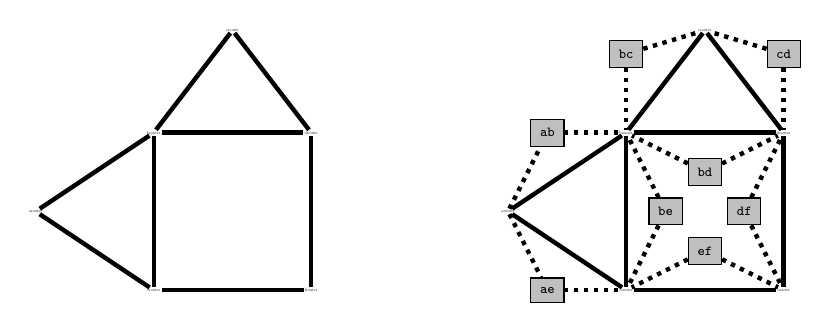
\begin{tikzpicture}
\def\dx{0}
%\node[draw, circle, fill=lightgray] (a) at (\dx + 0, 0) {\tiny \texttt{a}};
%\node[draw, circle, fill=lightgray] (b) at (\dx + 1, 1) {\tiny \texttt{b}};
%\node[draw, circle, fill=lightgray] (c) at (\dx + 2, 2) {\tiny \texttt{c}};
%\node[draw, circle, fill=lightgray] (d) at (\dx + 3, 1) {\tiny \texttt{d}};
%\node[draw, circle, fill=lightgray] (e) at (\dx + 1, -1) {\tiny \texttt{e}};
%\node[draw, circle, fill=lightgray] (f) at (\dx + 3, -1) {\tiny \texttt{f}};

\node[scale=0.15] (a) at (\dx + -0.5, 0) {\router{a}{router}};
\node[scale=0.15] (b) at (\dx + 1, 1) {\router{b}{router}};
\node[scale=0.15] (c) at (\dx + 2, 2.3) {\router{c}{router}};
\node[scale=0.15] (d) at (\dx + 3, 1) {\router{d}{router}};
\node[scale=0.15] (e) at (\dx + 1, -1) {\router{e}{router}};
\node[scale=0.15] (f) at (\dx + 3, -1) {\router{f}{router}};


\draw[ultra thick] (a) -- (b);
\draw[ultra thick] (a) -- (e);
\draw[ultra thick] (b) -- (e);
\draw[ultra thick] (b) -- (c);
\draw[ultra thick] (c) -- (d);
\draw[ultra thick] (b) -- (d);
\draw[ultra thick] (b) -- (e);
\draw[ultra thick] (f) -- (d);
\draw[ultra thick] (f) -- (e);

\def\dx{6}
%\node[draw, circle, fill=lightgray] (a) at (\dx + 0, 0) {\tiny \texttt{a}};
%\node[draw, circle, fill=lightgray] (b) at (\dx + 1, 1) {\tiny \texttt{b}};
%\node[draw, circle, fill=lightgray] (c) at (\dx + 2, 2) {\tiny \texttt{c}};
%\node[draw, circle, fill=lightgray] (d) at (\dx + 3, 1) {\tiny \texttt{d}};
%\node[draw, circle, fill=lightgray] (e) at (\dx + 1, -1) {\tiny \texttt{e}};
%\node[draw, circle, fill=lightgray] (f) at (\dx + 3, -1) {\tiny \texttt{f}};


\node[scale=0.15] (a) at (\dx + -0.5, 0) {\router{a}{router}};
\node[scale=0.15] (b) at (\dx + 1, 1) {\router{b}{router}};
\node[scale=0.15] (c) at (\dx + 2, 2.3) {\router{c}{router}};
\node[scale=0.15] (d) at (\dx + 3, 1) {\router{d}{router}};
\node[scale=0.15] (e) at (\dx + 1, -1) {\router{e}{router}};
\node[scale=0.15] (f) at (\dx + 3, -1) {\router{f}{router}};

\draw[ultra thick] (a) -- (b);
\draw[ultra thick] (a) -- (e);
\draw[ultra thick] (b) -- (e);
\draw[ultra thick] (b) -- (c);
\draw[ultra thick] (c) -- (d);
\draw[ultra thick] (b) -- (d);
\draw[ultra thick] (b) -- (e);
\draw[ultra thick] (f) -- (d);
\draw[ultra thick] (f) -- (e);

\node[draw, fill=lightgray] (ab) at (\dx + 0, 1) {\tiny \texttt{ab}};
\draw[ultra thick, dotted] (a) edge[above, sloped] (ab);
\draw[ultra thick, dotted] (b) edge[above, sloped] (ab);

\node[draw, fill=lightgray] (ae) at (\dx + 0, -1) {\tiny \texttt{ae}};
\draw[ultra thick, dotted] (a) edge[below, sloped] (ae);
\draw[ultra thick, dotted] (e) edge[below, sloped] (ae);

\node[draw, fill=lightgray] (bc) at (\dx + 1, 2) {\tiny \texttt{bc}};
\draw[ultra thick, dotted] (bc) edge[below, sloped] (b);
\draw[ultra thick, dotted] (bc) edge[below, sloped] (c);

\node[draw, fill=lightgray] (cd) at (\dx + 3, 2) {\tiny \texttt{cd}};
\draw[ultra thick, dotted] (cd) edge[below, sloped] (c);
\draw[ultra thick, dotted] (cd) edge[below, sloped] (d);

\node[draw, fill=lightgray] (bd) at (\dx + 2, 0.5) {\tiny \texttt{bd}};
\draw[ultra thick, dotted] (bd) edge[sloped] (b);
\draw[ultra thick, dotted] (bd) edge[sloped] (d);

\node[draw, fill=lightgray] (be) at (\dx + 1.5, 0) {\tiny \texttt{be}};
\draw[ultra thick, dotted] (be) edge[sloped] (b);
\draw[ultra thick, dotted] (be) edge[sloped] (e);

\node[draw, fill=lightgray] (ef) at (\dx + 2, -0.5) {\tiny \texttt{ef}};
\draw[ultra thick, dotted] (ef) edge[sloped] (e);
\draw[ultra thick, dotted] (ef) edge[sloped] (f);

\node[draw, fill=lightgray] (df) at (\dx + 2.5, 0) {\tiny \texttt{df}};
\draw[ultra thick, dotted] (df) edge[sloped] (d);
\draw[ultra thick, dotted] (df) edge[sloped] (f);

\end{tikzpicture}
\end{center}
\caption{Example of the transformation. Solid edges have weight $2$ whereas dotted edges have weight $2$.}
\label{fig-np-max-seg}
\end{figure}

Let $p$ be a path on $H$ from $s$ to $t$ such that $\cost(\mseg(p))$ is maximum. We start by proving that $p$
does not cross any of the new nodes, that is, only crosses nodes in $V(G) \cap V(H)$. Suppose that $p$ visits the node
sequence $(v_1, \ldots, v_l)$ and let $i$ be the smallest index such that $v_i \notin V(G)$. Since $p$ is a path from
$s$ to $t$ and $s, t \in V(G)$ we have that $1 < i < l$. Thus we can write $v_i = v_{i-1}v_{i+1}$ and 
$p = (v_1, \ldots, v_{i - 1}, v_i, v_{i + 1}, \ldots, v_l) = (v_1, \ldots, v_{i - 1}, v_{i - 1} v_{i+1}, v_{i +1} \ldots, v_l)$.
We need to consider three cases.

\emph{Case 1:} $v_{i + 2} \in V(G)$. In this case path $p$ has the form:

\begin{center}
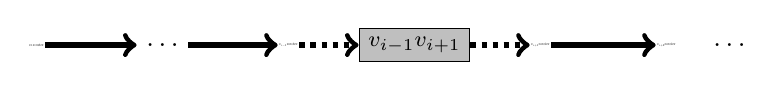
\begin{tikzpicture}[scale=0.8]
\node[scale=0.15] (v1) at (0, 0) {\router{$v_1$}{router}};
\node (dots) at (2, 0) {$\ldots$};
\node[scale=0.15] (vi-1) at (4, 0) {\router{$v_{i - 1}$}{router}};
\node[draw, fill=lightgray] (vi) at (6, 0) {\footnotesize $v_{i-1}v_{i+1}$};
\node[scale=0.15] (vi+1) at (8, 0) {\router{$v_{i + 1}$}{router}};
\node[scale=0.15] (vi+2) at (10, 0) {\router{$v_{i + 2}$}{router}};
\node (dots2) at (11, 0) {$\ldots$};

\draw (v1) edge[line width=2, ->] (dots);
\draw (dots) edge[line width=2, ->] (vi-1);
\draw (vi-1) edge[line width=2, dotted, ->] (vi);
\draw (vi) edge[line width=2, dotted, ->] (vi+1);
\draw (vi+1) edge[line width=2, ->] (vi+2);
\end{tikzpicture}
\end{center}

By construction, every link of $G$ that is traversed requires an adjacency segment
in its minimal segmentation (because of ECMP). 
Therefore, the minimal segmentation of this path is 
$$
\langle (v_1, v_2), (v_2, v_3), \ldots, (v_{i - 2}, v_{i - 1}), xy, (v_{i + 1}, v_{i + 2}), \ldots \rangle.
$$
On the other hand, if we remove element $xy$ from the path, we obtain a simple path $p'$ with the same minimal segmentation
except that $xy$ is replaced by the adjacency segment $(x, y)$ giving
$$
\langle (v_1, v_2), (v_2, v_3), \ldots, (v_{i - 2}, x), (x, y), (y, v_{i + 2}), \ldots \rangle.
$$
This segmentation costs one more than the segmentation of $p$. Since $p'$ is also a path from $s$ to $t$, this 
contradicts the fact that $p$ is a path from $s$ to $t$ that maximizes $\cost(\mseg(p))$.

\emph{Case 2:} $v_{i + 2} \notin V(G)$. In this case, $p$ has the following form:

\begin{center}
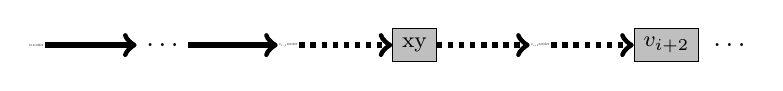
\begin{tikzpicture}[scale=0.8]
\node[scale=0.15] (v1) at (0, 0) {\router{$v_1$}{router}};
\node (dots) at (2, 0) {$\ldots$};
\node[scale=0.15] (vi-1) at (4, 0) {\router{$v_{i - 1}$}{router}};
\node[draw, fill=lightgray] (vi) at (6, 0) {\footnotesize xy};
\node[scale=0.15] (vi+1) at (8, 0) {\router{$v_{i + 1}$}{router}};
\node[draw, fill=lightgray] (vi+2) at (10, 0) {\footnotesize $v_{i + 2}$};
\node (dots2) at (11, 0) {$\ldots$};

\draw (v1) edge[line width=2, ->] (dots);
\draw (dots) edge[line width=2, ->] (vi-1);
\draw (vi-1) edge[line width=2, dotted, ->] (vi);
\draw (vi) edge[line width=2, dotted, ->] (vi+1);
\draw (vi+1) edge[line width=2, dotted, ->] (vi+2);
\end{tikzpicture}
\end{center}

The minimal segmentation of $p$ will be
$$
\langle (v_1, v_2), (v_2, v_3), \ldots, (v_{i - 2}, x), xy, v_{i + 2}, \ldots \rangle.
$$
As before, if we remove $xy$ from $p$ we obtain a simple path $p'$ from $s$ to $t$
with minimal segmentation equal to
$$
\langle (v_1, v_2), (v_2, v_3), \ldots, (v_{i - 2}, x), (x, y), v_{i + 2}, \ldots \rangle.
$$
This segmentation costs one more than the minimal segmentation of $p$ so as above, we conclude
that $p$ does not minimize $\cost(\mseg(p))$.

These two cases cover all possibilities so we conclude that the path $p$ on $H$ that maximizes
$\cost(\mseg(p))$ has all of its nodes in $V(G)$. Therefore, this is also a path in $G$.
Furthermore, because of ECMP, that the minimal segmentation of $p$ will contain
all of its edges as adjacency segments. Hence $\cost(\mseg(p)) = 2 |E(p)|$ so it follows that
if can find a path on $H$ that maximizes $\cost(\mseg(p))$ we can find a path on $G$ that maximizes
$E(p)$ which completes the proof.
% 
% 
% \newpage
% 
% Let $p = (v_1, v_2, \ldots, v_k)$ be a simple path in $G$. By theorem \todo{adjacency segment theorem}, each edge of path $p$
% requires an adjacency segment. Therefore, $\mseg(p) = \langle (v_1, v_2), (v_2, v_3), \ldots, (v_{k - 1}, v_k) \rangle$.
% 
% Let $p = (u_1, u_2, \ldots, u_k)$ be a path in $H$ such that $\cost(\mseg(p))$ is maximum. We are going to prove that
% there exists a path $q$ containing only nodes in $V(G)$ with the same segmentation cost.
% 
% 
% If $u_i \in V(G)$ for each $i = 1, \ldots, k$ then there is noting to prove. Othersiwe, let $i$ by the minimum index
% such that $u_i \notin V(G)$. Write $u_i = xy$ where $x, y \in V(G)$.
% 
% Then $p$ has the form $(u_1, \ldots, u_{i - 1}, u_i, u_{i + 1} \ldots) = (u_1, \ldots, x, xy, y, \ldots)$.
% The minimal segmentation of $p$ must has the form $\langle (u_1, u_2), (u_2, u_3), \ldots, (u_{i - 1}, x), \ldots, \rangle$
% 
% The minimal segmentation $\sr{p}$ of $p$ on $H$ is easy to characterize. 
% It will contain all special nodes $u_i \notin V(G)$ as node segments
% together with all edges $(u_i, u_{i + 1}) \in E(G)$ as adjacency segemnts (in their order of appearence). Finally,
% if $(u_1, u_2) \notin E(G)$ then $u_1$ will apprear as the first node and if $(u_{k - 1}, u_k) \notin E(G)$, then $u_k$
% will appear as the last node.
% 
% Therefore, if we remove the first special node $u_i \notin V(G)$ from $p$
% 
% \todo{STEPS:
% \begin{itemize}
%  \item Prove the structure of minimal segmentations on $H$
%  \item Prove that we can replace the first special node $ab$ by $b$. 
%  We need to make sure that the segment cost is not reduced and that we still have a simple path.
%  \item With this we show that there exists a solution of the problem that is a path in $G$.
%  \item We show that any path in $G$ maps to a path in $H$ with double segment cost.
%  \item We conclude that if there was a longer path in $G$ then we would have a longer segmentation
% \end{itemize}
% }
% 
% For instance, path $(a, ab, b, bc, c, d)$ has minimal segmentation $\langle a, ab, bc, (c, d) \rangle$.

\end{proof}

\begin{corollary}
Problem \ref{prob:max-seg} is \NPhard. 
\end{corollary}

\begin{proof}
Let $G, s, t$ be an instance of Problem \ref{prob:max-seg-st}. 
%We will build an instance $G'$ of Problem \ref{prob:max-seg}
%whose answer is the optimal solution of Problem \ref{prob:max-seg-st} plus some constant $C$. 
Let $m = E(G)$. We build a graph by adding a path $(x_1, \ldots, x_m, s)$ connecting to $s$ whose minimal segmentation 
has segment cost $2 m$ and a path $(t, y_1, \ldots, y_m)$ going out of $t$ whose minimal segmentation also has segment cost
$2 m$. This is achieved by adding also nodes $x'_1, \ldots, x'_m$ and $y'_1, \ldots, y'_m$ and edges $(x_i, x'_i)$ and
$(x'_i, x_{i + 1})$ of cost $1$ to ensure that adjacency segments are required to segment the two paths
mentioned above. Figure \ref{fig:np-transform2} illustrates this. Dashed edges represent edges of cost $1$
and solid edges represent edge of cost $2$.

\begin{figure}[H]
\begin{center}
\begin{tikzpicture}[scale=0.8]
\draw[ultra thick, lightgray, fill=lightgray!50!white] (0, 0) circle (2);
\node[scale=0.15] (s) at (-0.75, -0.75) {\router{$s$}{router}};
\node[scale=0.15] (t) at (0.75, 0.75) {\router{$t$}{router}};
\node[] (g) at (-1, 1) {$G$};

\node (gg) at (-5, 2) {$G'$};

\node[scale=0.15] (xm) at (-2.5, -0.75) {\router{$x_m$}{router}};
\node[scale=0.15] (xxm) at (-2.5, -3) {\router{$x'_m$}{router}};
\node[scale=0.15] (xm-1) at (-4.5, -0.75) {\router{$x_{m - 1}$}{router}};
\node[scale=0.15] (xxm-1) at (-4.5, -3) {\router{$x'_{m-1}$}{router}};
\node at (-5.5, -0.75) {$\ldots$};
\node[scale=0.15] (x1) at (-6.5, -0.75) {\router{$x_{1}$}{router}};
\node[scale=0.15] (xx1) at (-6.5, -3) {\router{$x'_{1}$}{router}};

\draw (xm) edge[line width=2, dotted, ->] (xxm);
\draw (xxm) edge[line width=2, dotted, ->] (s);
\draw (xm) edge[line width=2, ->] (s);

\draw (xm-1) edge[line width=2, dotted, ->] (xxm-1);
\draw (xxm-1) edge[line width=2, dotted, ->] (xm);
\draw (xm-1) edge[line width=2, ->] (xm);
\draw (x1) edge[line width=2, ->, dotted] (xx1);

\node[scale=0.15] (ym) at (2.5, 0.75) {\router{$y_m$}{router}};
\node[scale=0.15] (yym) at (2.5, 3) {\router{$y'_m$}{router}};
\node[scale=0.15] (ym-1) at (4.5, 0.75) {\router{$y_{m - 1}$}{router}};
\node[scale=0.15] (yym-1) at (4.5, 3) {\router{$y'_{m-1}$}{router}};
\node at (5.5, 0.75) {$\ldots$};
\node[scale=0.15] (y1) at (6.5, 0.75) {\router{$y_{1}$}{router}};
\node[scale=0.15] (yy1) at (6.5, 3) {\router{$y'_{1}$}{router}};


\draw (ym) edge[line width=2, dotted, <-] (yym);
\draw (yym) edge[line width=2, dotted, <-] (t);
\draw (ym) edge[line width=2, <-] (t);

\draw (ym-1) edge[line width=2, dotted, <-] (yym-1);
\draw (yym-1) edge[line width=2, dotted, <-] (ym);
\draw (ym-1) edge[line width=2, <-] (ym);
\draw (y1) edge[line width=2, <-, dotted] (yy1);

\draw[cyan, line width=2, ->] plot [smooth] coordinates { ($(x1)+(0,0.5)$) ($(xm-1)+(0,0.5)$) ($(xm)+(0,0.5)$)  ($(s)+(0,0.5)$) ($(s)+(0.5,0.5)$) ($(t)+(0,-0.5)$) ($(ym)+(0,-0.5)$) ($(ym-1)+(0,-0.5)$) ($(y1)+(0,-0.5)$)};



\end{tikzpicture}
\end{center}
\caption{Example of the transformation.}
\label{fig:np-transform2}
\end{figure}

By lemma \ref{lemma:edgeseg}, the maximum cost of a minimal segmentation in $G$ is at most $2 m$. Therefore,
the maximum cost of a minimal segmentation of a path in $G'$ must be a path from $x_1$ to $y_1$ since just this part
of the path will have segment cost at least $4m$. Since the path from $x_1$ passes by $s$, to each
$y_1$ we need to pass by $t$, we will achieve the maximum segment cost by connecting $s$ and $t$ by path with maximum 
segmentation cost. Thus the solution to Problem \ref{prob:max-seg} on $G'$ is a path of cost $x + 4m$ where $x$ is the cost of
the solution to problem \ref{prob:max-seg-st} on input $G, s, t$. We conclude that if we could solve Problem \ref{prob:max-seg}
in polynomial time then we could also solve Problem \ref{prob:max-seg-st} in polynomial time. Therefore, by Theorem \ref{thm:max-seg-st-np},
we conclude that \ref{prob:max-seg} is \NPhard.


\end{proof}



% ------------------------------------------------------------
% 
% \todo{this needs to be fixed, it still uses $\ereach(2, v)$ assuming that it mean unique shortest path}
% 
% \begin{theorem}
% \label{thm:ereach}
% Let $G$ be a network, $s \in V(G)$ and an integer $k \geq 3$. It holds that
% \begin{align*}
% \ereach(1, s) = & \ \emptyset \\
% \ereach(2, s) = & \ \{ e \in E(G) \mid \sp(s, v) \textrm{ is a path with last edge $e$} \} \quad \cup \\
%                 & \ \{ (s, u) \mid (s, u) \in E(G) \} \\
% \ereach(k, s) = & \ \bigcup_{v \in \nreach(k - 1, s)} \ereach(2, v) \quad \cup \\ 
% & \ \bigcup_{v \in \nreach(k - 2, s)}  \left\{ (u_1, u_2) \mid (u_1, u_2) \in E(G) \wedge u_1 \in \nreach(2, v) \right\}
% \end{align*}
% \end{theorem}
% 
% \begin{proof}
% For $k = 1$ the only sr-path of cost $1$ starting from $s$ is $\langle s \rangle$ and it contains no edges. Thus $\nreach(1, s) = \emptyset$.
% For $k = 2$, a sr-path of cost $2$ starting at $s$ has either the form $\langle s, v \rangle$ where
% $v \in V(G)$ or $\langle (s, v) \rangle$ where $(s, v) \in E(G)$. Thus, for each $v$ such that $\sp(s, v)$ is a path,
% the last edge will belong to $\ereach(2, s)$. Also, every edge of the form $(s, v)$ will belong to $\ereach(2, s)$
% 
% Let $k \geq 3$.
% 
% $(\subseteq)$ Let $e \in \ereach(k, v)$. Then there exists a deterministic sr-path 
% $\sr{p} = \langle x_1, \ldots, x_{l - 1}, x_l \rangle$  of segment cost at most $k$ such that
% either $x_l = e$ or $x_l$ is a node
% segment and $e$ is the last edge of the unique shortest path between $x^2_{l - 1}$
% and $x_{l}$. Let $\sr{q} = \langle x_1, \ldots x_{l - 1} \rangle$ and $v = x^2_{l - 1}$.
% 
% \emph{Case 1:} $x_l = e = (u_1, u_2)$. Let 
% Since $\cost(\sr{p}) \leq k$, we know that
% $\cost(\sr{q}) \leq k - 2$. Thus $v = x^2_{l - 1} \in \nreach(k - 2, s)$. 
% Since $\sr{p}$ is deterministic, 
% there must be a unique shortest path
% between $x^2_{l - 1} = v$ to $x^1_l = u_1$. Therefore, $u_1 \in \nreach(2, v)$ so
% $$
% e \in \bigcup_{v \in \nreach(k - 2, s)}  \left\{ (u_1, u_2) \mid (u_1, u_2) \in E(G) \wedge u_1 \in \nreach(2, v) \right\}.
% $$
% 
% \emph{Case 2:} $x_l$ is a node segment and $e$ is the last edge of the unique
% shortest path between $x^2_{l - 1}$ and $x_l$. Then $\cost(\sr{q}) \leq k - 1$
% so that $v \in \nreach(s, k - 1)$. Since $e$ is the last edge of the unique
% shortest path between $v = x^2_{l - 1}$ and $x_l$ we have that $e \in \ereach(2, v)$.
% Thus
% $$
% e \in \bigcup_{v \in \nreach(k - 1, s)} \ereach(2, v).
% $$
% 
% $(\supseteq)$ Let $e \in \bigcup_{v \in \nreach(k - 1, s)} \ereach(v, 2)$. Then
% there exists $v \in \nreach(k - 1, s)$ such that $e \in \ereach(v, 2)$. By definition,
% this means that there exists a deterministic sr-path $\sr{p} = \langle x_1, \ldots, x_l \rangle$
% from $s$ to $v$ with $\cost(\sr{p}) \leq k - 1$ and a unique shortest path from $v$ to $u$
% such that $e$ is the last edge of that path. Thus, $\langle x_1, \ldots, x_l, u \rangle$ is a deterministic
% sr-path from $s$ to $u$ of cost at most $k - 1 + 1 = k$ with last edge $e$. We conclude that
% $e \in \ereach(s, k)$.
% 
% Let $(u_1, u_2) \in \bigcup_{v \in \nreach(k - 2, s)}  \left\{ (u_1, u_2) \mid (u_1, u_2) \in E(G) \wedge u_1 \in \nreach(2, v) \right\}$.
% Then there exists $v \in \nreach(k - 2, s)$ such that $u_1 \in \nreach(2, v)$. 
% By definition, this means that we have a deterministic sr-path $\sr{p} = \langle x_1, \ldots, x_l \rangle$ from $s$ to $v$ with segment cost at most $k - 2$ and
% a unique shortest path from $v$ to $u_1$. Therefore $\langle x_1, \ldots, x_l, (u_1, u_2) \rangle$ is a deterministic sr-path
% from $s$ to $u_2$ of segment cost at most $k - 2 + 2 = k$ with last element being an adjacency segment
% on $(u_1, u_2)$. Hence, $(u_1, u_2) \in \ereach(k, s)$.
% \end{proof}


% \begin{proposition}
% Let $G$ be a network, $s \in V(G)$. Then for $k \geq 2$,
% \begin{align*}
% \nreach(0, s) = & \left\{ s \right\} \\
% \nreach(1, s) = & \left\{ V(\sp(s, v)) \mid \textrm{$v \in V(G)$ and $\sp(s, v)$ is a path} \right\} \\
% \nreach(k, s) = & \bigcup_{v \in \nreach(k - 1, s)} \nreach(1, v) \quad \cup \\
%                 & \left\{ u_2 \mid (u_1, u_2) \in E(G) \wedge \exists u \in \nreach(k - 2, s) : u_1 \in \nreach(1, u) \right\}
% \end{align*}
% \end{proposition}
% 
% \begin{proof}
% If $k = 0$ then the only sr-path starting at $s$ of segment cost at most $0$ is $\langle s \rangle$. Thus, since $V(\langle s \rangle) = s$, $\nreach(0, s) = \{ s \}$.
% For $k = 1$, the sr-paths starting at $s$ with segments cost at most $1$ are for the form $\langle s, v \rangle$ for $v \in V(G)$. From these, we only consider the ones
% that are deterministic, that is, the ones such that there is a unique shortest path between $s$ and $v$. In other words, the ones such that $\sp(s, v)$ is a path.
% 
% For $k \geq 2$ we will prove the that each set is contained inside the other. 
% 
% $(\subseteq)$ Let $v \in \nreach(k, s)$. Then, by definition, there exists a deterministic sr-path $\sr{p} = \langle x_1, \ldots, x_l \rangle$
% of cost at most $k$ such that $v \in V(\sr{p})$.
% \end{proof}




% \section{SR formalization}
% 
% In this section we propose a mathematical formalization of segment routing. This is a first step
% towards a uniformisation of the mathematical notations used to represent segments routing problems.
% 
% \todo{more blabla}
% 
% The first thing tht we are going to define are the concepts of node and adjacency segments.
% 
% \begin{definition}
% Let $G$ be a network. We define the \emph{segment set} of $G$ as $\seg(G) = V(G) \cup E(G)$.
% Let $x \in \seg(G)$. If $x = (u, v) \in E(G)$ we write $x^- = u$ and $x^+ = v$.
% Otherwise $x = v \in V(G)$ and we write $x^- = x^+ = v$.
% \end{definition}
% 
% Note that even for node segments we define the notations $x^-$ and $x^+$. As we will see shortly,
% it makes it possible to express other concept in a much more elegent maner as it avoids having
% to distinguish between the times of segments that are under consideration.
% 
% Next, we define the concept of segment routing paths, which essentially capture the segment
% stack that will be provided to the ingress node. The main difference between this definition and the
% ingress node is considered to be part of the path whereas in real netwoks it is not added to the SR stack.
% 
% \begin{definition}
% A \emph{segment routing path (sr-path)} is a sequence $\sr{p} = \langle x_1, \ldots, x_k \rangle$ such that each $x_i \in \seg(G)$ and
% for each $i = 2, \ldots k$, $x^+_{i - 1} \rightsquigarrow x^-_i$. We call $k$ the \emph{length} of $\sr{p}$ and write $\len(\sr{p}) = k$.
% 
% We write $\node(\sr{p}) = \{ x_i \mid x_i \in V(G) \}$ and call its elements \emph{node segments} and $\adj(\sr{p}) = \{ x_i \mid x_i \in E(G) \}$
% and call its elements \emph{adjacency segments}.
% 
% Finally, we define the \emph{segment cost} of $\sr{p}$ as $|\node(\sr{p})| + 2 \cdot |\adj(\sr{p})|$. We write it as $\cost(\sr{p})$.
% \end{definition}
% 
% The reason why adjacency segments have a double weight on the segment cost is because they require two entries in the segment
% stack instead of one. The segment cost is a huge constraint for SR as most routers have a very limited SR stack size \todo{ref}.
% 
% As we saw in the introduction, packets forwarded on a sr-path will follow shortest paths between consecutive segments. It can
% happen that more than one shortest path exists between to consecutive segments. This is called Equal-Cost MultiPath (ECMP) in the
% networking literature \todo{ref}. In this case, depending on the underlying
% application, one of two things can happend: (i) the traffic is split in some way among all those paths for load balancing or (ii)
% a single one of those paths is used to forward the traffic and this selection is done using a hash function. \todo{ref?} In the later case,
% the network operators have no way of knowing apriori which of them will be used.
% 
% In any case, we need a  way to describe all the network links that can contribute to the forwarding of packets between
% two consecutive segments. This leads to the definition of forwarding graphs.
% 
% \begin{definition}
% Let $\sr{p} = \langle x_1, \ldots, x_k \rangle$ be a sr-path. We define the \emph{forwarding graph} of $\sr{p}$ by
% $$
% \forw(\sr{p}) = \left( \bigcup_{i = 2}^k \sp(x^+_{i - 1}, x^-_{i}) \right) \cup \bigcup_{x \in \adj(\sr{p})} x.
% $$
% \end{definition}
% 
% The first part of the defintion of forwarding graphs captures all the shortest paths that are used between consecutive segments
% and the second part captures all links represented by adjacency segments. To better illustrate this defintion let's consider a few examples.
% 
% Figure \ref{fig:sr1} shows, in green, $\forw(\langle a, (d, e), i \rangle)$. To see that it matches the definition, we can write
% \begin{align*}
% \forw(\langle a, (d, e), i \rangle) & = \sp(a^+, (d, e)^-) \cup \sp( (d, e)^+, i^-) \cup (d, e) \\
% & = \sp(a, d) \cup \sp(e, i) \cup (d, e) \\
% & = (a, c, d) \cup (e, h, i) \cup (d, e) \\
% & = \{ (a, c), (c, d), (e, h), (h, i), (d, e) \}.
% \end{align*}
% 
% Consider now the sr-path $\sr{p} = \langle a, b, (d, e), i \rangle$ on the same graph as shown in Figure \ref{fig:sr2}. This
% example illustrates two things. First, from $b$ to the origin of $(d, e)$ there are two shortest paths so we see that
% $\forw(\sr{p})$ corresponds to a subgraph of $G$ and not just a path. Second, we see that the forwarding subgraph can
% contain cycles contrary to what our intuition might suggest. To confirm that this is correct we compute $\forw(\sr{p})$
% once more:
% \begin{align*}
% \forw(\langle a, b, (d, e), i \rangle) & = \sp(a^+, b^-) \cup \sp( b^+, (d, e)^-) \cup \sp( (d, e)^+, i^-) \cup (d, e) \\
% & = \sp(a, b) \cup \sp(b, e) \cup \sp(e, i) \cup (d, e) \\
% & = (a, b) \cup (b, c, d) \cup (b, e, d) \cup (e, h) \cup (h, i) \cup (d, e) \\
% & = \{ (a, b) (b, c), (c, d), (b, e), (e, d), (e, h), (h, i), (d, e) \}.
% \end{align*}
% 
% 
% \begin{figure}[H]
% \begin{center}
% \begin{tikzpicture}
% \def\x{0}
% \def\y{0}
% \node[scale=0.15] (a) at (0.5 + \x,  0.5 + \y) {\router{a}{green}};
% \node[scale=0.15] (b) at (0.5 + \x, -1.0 + \y) {\router{b}{green}};
% \node[scale=0.15] (c) at (2.5 + \x,  0.0 + \y) {\router{c}{lightgray}};
% \node[scale=0.15] (d) at (4.5 + \x,  0.0 + \y) {\router{d}{green}};
% \node[scale=0.15] (e) at (4.0 + \x, -2.0 + \y) {\router{e}{green}};
% \node[scale=0.15] (g) at (6.0 + \x,  0.5 + \y) {\router{g}{lightgray}};
% \node[scale=0.15] (i) at (8.0 + \x,  0.0 + \y) {\router{i}{green}};
% \node[scale=0.15] (h) at (7.0 + \x, -1.5 + \y) {\router{h}{lightgray}};
% \node[scale=0.15] (f) at (4.0 + \x, -3.5 + \y) {\router{f}{lightgray}};
% \node[scale=0.15] (j) at (8.0 + \x, -2.5 + \y) {\router{j}{lightgray}};
% \draw[line width=2] (f) edge[above, sloped] node[black,font=\bfseries] {\tiny \texttt{}} (j);
% \draw[line width=2] (h) edge[above, sloped] node[black,font=\bfseries] {\tiny \texttt{}} (j);
% \draw[line width=2] (a) edge[above, sloped] node[black,font=\bfseries] {\tiny \texttt{}} (b);
% \draw[line width=2] (b) edge[above, sloped] node[black,font=\bfseries] {\tiny \texttt{}} (c);
% \draw[line width=2] (e) edge[above, sloped] node[black,font=\bfseries] {\tiny \texttt{}} (c);
% \draw[line width=2] (b) edge[above, sloped] node[black,font=\bfseries] {\tiny \texttt{}} (e);
% \draw[line width=2] (b) edge[above, sloped] node[black,font=\bfseries] {\tiny \texttt{}} (f);
% \draw[line width=2] (e) edge[above, sloped] node[black,font=\bfseries] {\tiny \texttt{}} (f);
% \draw[line width=2] (h) edge[above, sloped] node[black,font=\bfseries] {\tiny \texttt{}} (f);
% \draw[line width=2] (g) edge[above, sloped] node[black,font=\bfseries] {\tiny \texttt{}} (i);
% \draw[line width=2] (i) edge[above, sloped] node[black,font=\bfseries] {\tiny \texttt{}} (h);
% \draw[line width=2]  (d) edge[above, sloped] node[black,font=\bfseries] {\tiny \texttt{}} (g);
% \draw[line width=2]  (d) edge[above, sloped] node[black,font=\bfseries] {\tiny \texttt{}} (e);
% \draw[line width=2]  (e) edge[above, sloped] node[black,font=\bfseries] {\tiny \texttt{}} (h);
% \draw[line width=2]  (g) edge[above, sloped] node[black,font=\bfseries] {\tiny \texttt{}} (h);
% \draw[line width=2]  (c) edge[above, sloped] node[black,font=\bfseries] {\tiny \texttt{}} (d);
% \draw[line width=2]  (a) edge[above, sloped] node[black,font=\bfseries] {\tiny \texttt{}} (b);
% \draw[line width=2]  (a) edge[above, sloped] node[black,font=\bfseries] {\tiny \texttt{}} (c);
% 
% %%%%
% \draw (a) edge[line width=2, darkgreen, above, ->, bend right = 20] (b);
% \draw (b) edge[line width=2, darkgreen, above, ->, bend left = 20] (c);
% \draw (b) edge[line width=2, darkgreen, above, ->, bend left = 20] (e);
% \draw (e) edge[line width=2, darkgreen, above, ->, bend left = 30] (d);
% \draw (c) edge[line width=2, darkgreen, above, ->, bend left = 20] (d);
% \draw (d) edge[line width=2, darkgreen, above, ->, dotted] (e);
% \draw (e) edge[line width=2, darkgreen, above, ->, bend left = 20] (h);
% \draw (h) edge[line width=2, darkgreen, above, ->, bend left = 20] (i);
% 
% 
% \def\x{-0.5}
% \def\y{1}
% \node at (\x + 2.7, \y + 0.25) {\footnotesize SR stack};
% \fill[lightgray] (\x, \y) rectangle (\x + 2, \y + 0.5);
% \fill[green] (\x, \y) rectangle (\x + 0.5, \y + 0.5);
% \draw[dotted, thick] (\x + 0.7, \y) -- (\x + 0.7, \y - 0.4);
% \draw[] (\x, \y) rectangle (\x + 2, \y + 0.5);
% \draw (\x + 0.5, \y) -- (\x + 0.5, \y + 0.5);
% \draw (\x + 1.5, \y) -- (\x + 1.5, \y + 0.5);
% \node at (\x + 0.25, \y + 0.26) {\footnotesize $b$};
% \node at (\x + 1, \y + 0.25) {\footnotesize $(d, e)$};
% \node at (\x + 1.75, \y + 0.28) {\footnotesize $i$};
% 
% 
% \def\x{-0.5}
% \def\y{-2}
% \fill[lightgray] (\x, \y) rectangle (\x + 2, \y + 0.5);
% \fill[gray] (\x, \y) rectangle (\x + 0.5, \y + 0.5);
% \fill[green] (\x + 0.5, \y) rectangle (\x + 1.5, \y + 0.5);
% \draw[dotted, thick] (\x + 0.7, \y + 0.5) -- (\x + 0.7, \y + 0.8);
% \draw[] (\x, \y) rectangle (\x + 2, \y + 0.5);
% \draw (\x + 0.5, \y) -- (\x + 0.5, \y + 0.5);
% \draw (\x + 1.5, \y) -- (\x + 1.5, \y + 0.5);
% \node at (\x + 0.25, \y + 0.26) {\footnotesize $b$};
% \node at (\x + 1, \y + 0.25) {\footnotesize $(d, e)$};
% \node at (\x + 1.75, \y + 0.28) {\footnotesize $i$};
% 
% 
% \def\x{3}
% \def\y{-3}
% \fill[lightgray] (\x, \y) rectangle (\x + 2, \y + 0.5);
% \fill[gray] (\x, \y) rectangle (\x + 1.5, \y + 0.5);
% \fill[green] (\x + 1.5, \y) rectangle (\x + 2, \y + 0.5);
% \draw[dotted, thick] (\x + 0.7, \y + 0.5) -- (\x + 0.7, \y + 0.8);
% \draw[] (\x, \y) rectangle (\x + 2, \y + 0.5);
% \draw (\x + 0.5, \y) -- (\x + 0.5, \y + 0.5);
% \draw (\x + 1.5, \y) -- (\x + 1.5, \y + 0.5);
% \node at (\x + 0.25, \y + 0.26) {\footnotesize $b$};
% \node at (\x + 1, \y + 0.25) {\footnotesize $(d, e)$};
% \node at (\x + 1.75, \y + 0.28) {\footnotesize $i$};
% 
% \def\x{8 - 0.75 - 0.25}
% \def\y{0.5}
% \fill[lightgray] (\x, \y) rectangle (\x + 2, \y + 0.5);
% \fill[gray] (\x, \y) rectangle (\x + 2, \y + 0.5);s
% \draw[dotted, thick] (\x + 0.7, \y) -- (\x + 0.7, \y - 0.4);
% \draw[] (\x, \y) rectangle (\x + 2, \y + 0.5);
% \draw (\x + 0.5, \y) -- (\x + 0.5, \y + 0.5);
% \draw (\x + 1.5, \y) -- (\x + 1.5, \y + 0.5);
% \node at (\x + 0.25, \y + 0.26) {\footnotesize $b$};
% \node at (\x + 1, \y + 0.25) {\footnotesize $(d, e)$};
% \node at (\x + 1.75, \y + 0.28) {\footnotesize $i$};
% 
% 
% %%%%
% 
% %\def\x{-1}
% 
% %\draw[line width=2] (\x + 10, \y + -1 + 0.5) edge[] (\x + 10.5, \y + -1 + 0.5);
% %\node[anchor=west]  at (\x + 10.5, \y + -1 + 0.5) {\footnotesize network link};
% 
% %\draw[line width=2] (\x + 10, \y + -1) edge[dotted, darkgreen, ->] (\x + 10.5, \y + -1);
% %\node[anchor=west]  at (\x + 10.5, \y + -1) {\footnotesize adjacency segment};
% 
% %\draw[line width=2] (\x + 10, \y + -1 - 0.5) edge[] (\x + 10.5, \y + -1 - 0.5);
% %\node[anchor=west]  at (\x + 10.5, \y + -1 - 0.5) {\footnotesize s link};
% 
% 
% \end{tikzpicture}
% \end{center}
% \label{fig:sr2}
% \caption{Illustration of SR with segments $b$, $(d, e)$ and $i$ and ingress node $a$. Dashed arrows represent adjacency segments
% and the others represent the shortest path edges between consecutive segments.}
% \end{figure}
% 
% Consider the path $p = (a, b, c, d)$. We have that both sr-paths $\sr{p} = \langle a, b, c, d \rangle$  and $\sr{q} = \langle c, d, a, b \rangle$ 
% satisfy $\forw(\sr{p}) = \forw(\sr{q}) = p$. However, only $\sr{p}$ respects the order of visited nodes of $p$ meaning that even though
% $\sr{q}$ is a segmentation of $q$, it does not faithfully represent $p$ from a traffic forwarding standpoint.
% 
% \begin{center}
% \begin{tikzpicture}
% \node[scale=0.15] (a) at (0, 0) {\router{a}{lightgray}};
% \node[scale=0.15] (b) at (2, 0) {\router{b}{lightgray}};
% \node[scale=0.15] (c) at (2, 2) {\router{c}{lightgray}};
% \node[scale=0.15] (d) at (0, 2) {\router{d}{lightgray}};
% 
% \draw[line width=2] (a) edge[above, sloped] node[black,font=\bfseries] {\tiny \texttt{}} (b);
% \draw[line width=2] (b) edge[above, sloped] node[black,font=\bfseries] {\tiny \texttt{}} (c);
% \draw[line width=2] (c) edge[above, sloped] node[black,font=\bfseries] {\tiny \texttt{}} (d);
% \draw[line width=2] (d) edge[above, sloped] node[black,font=\bfseries] {\tiny \texttt{}} (a);
% 
% \end{tikzpicture}
% \end{center}
% 
